\documentclass[12pt,a4paper]{report}
\usepackage{graphicx}
\usepackage{amsmath}
\usepackage{fancyhdr}
\usepackage{cite}
\usepackage{framed}
\usepackage{a4wide}
\usepackage{float}
\usepackage{epsfig}
\usepackage{longtable}
\usepackage{enumerate}
\usepackage{afterpage}
\usepackage{multirow}
\usepackage{ragged2e}
\usepackage{gensymb}
\usepackage{amsfonts} 
\usepackage[left=2.2cm,top=1.5cm,right=2.2cm,bottom=4cm]{geometry}
\usepackage{setspace}           
\usepackage{float}
\usepackage{txfonts}
\usepackage{lipsum}
\usepackage{titlesec}
\usepackage{chngcntr}
\counterwithin{section}{chapter}
\counterwithin{subsection}{section}

\newcommand{\Usefont}[1]{\fontfamily{#1}\selectfont}

\usepackage{lscape} % for landscape tables
\renewcommand{\baselinestretch}{1.7} 

\usepackage{blindtext}
\usepackage{xpatch}
\usepackage{url}
\usepackage{leqno}
\usepackage{subcaption}

\linespread{1.5}
\usepackage[intoc, english]{nomencl}
\hyphenpenalty=5000
\tolerance=1000
\usepackage[nottoc]{tocbibind}

% ******* References config *********
\bibliographystyle{IEEEtran}   % On some TeX systems this works
%\bibliographystyle{ieeetr}      % While on others this works
							% Uncomment and test if your references don't cite
							% correctly
\renewcommand{\bibname}{References}

%*******************************************************************
%                        Header and Footer   
% This is not required in Technical reports submitted to CET ECE department.
% Please leave it commented                       
%*******************************************************************
%\pagestyle{fancy}
%\fancyhead{}
%\header and footer section
%\renewcommand\headrulewidth{0.1pt}
%\fancyhead[L]{\footnotesize \leftmark}
%\fancyhead[R]{\footnotesize \thepage}
%\renewcommand\headrulewidth{0pt}
%\fancyfoot[R]{\small College of Engineering Trivandrum}
%\renewcommand\footrulewidth{0.1pt}
%\fancyfoot[C]{2020 - 2021}
%\fancyfoot[L]{\small Title of the Seminar/Project}
%*******************************************************************


%*********************Figures*****************************
% Save all figures in the folder figures and include them in your 
% report using the command \includegraphics{figure-name}

\graphicspath{{figures/}}

% figure files can be in jpeg,jpg, png or pdf formats
%*******************************************************************
\titleformat{\chapter}[display]
  {\normalfont\bfseries}{}{0pt}{\Huge}
\titlespacing*{\chapter}{0pt}{0pt}{20pt} % Set spacing values to 0pt % Adjust the spacing values as needed
% Reset counters for figures and tables
\counterwithout{figure}{chapter}
\counterwithout{table}{chapter}
\begin{document}
	
	
%****The entries in this section are to be filled in by the student with appropriate values *************

% These values are used thoroughout the report 
% please fill in the appropriate values

\gdef \title{Seminar title} % Seminar title
\gdef \author{Student Name}	 %student name
\gdef \dept{Computer Science and Engineering} %Department
\gdef \degree{Bachelor of Technology} %degree
\gdef \branch{Computer Science and Engineering} %branch
\gdef \college{TKM College of Engineering}
\gdef \collegeplace{Kollam}
\gdef \rollno{TKM20CS0--} %KTU Reg No
\gdef \deptabbr{Dept.of CSE} %Dept name abbreviation

\gdef \guide{Prof. Thushara A} %Seminar guide
\gdef \guidedes{Associate Professor}%Seminar guide designation

\gdef \semcordinatorA{Prof. Thushara A}% Seminar coordinator 1 
\gdef \semcordinatorAdes{Associate Professor}% Seminar coordinator 1 designation

\gdef \semcordinatorB{Prof. Thushara A} % Seminar coordinator 2 
\gdef \semcordinatorBdes{Associate Professor}% Seminar coordinator 2 designation

\gdef \hod{Dr.Dimple A Shajahan} %Head of Department
\gdef \hoddes{Professor} %HOD designation

\gdef \acadyear{2023-2024} % Academic year
\gdef \month{December 2023} %Month of Report submission
\gdef \date{07-12-2023} %Date of signing the declaration

%*******************************************************************
% The font pages. The source tex files are there in the folder
%==================================coverpage.tex================================


\newenvironment{coverpage}
\thispagestyle{empty}
\begin{titlepage}
	\begin{center}
		{\Usefont{phv} \Large \bf \title \par}
		\vspace*{40pt}
		\large \em \Usefont{pzc}{ 
			A Seminar Report \par
			Submitted to the APJ Abdul Kalam Technological University\\
			in partial fulfillment of requirements for the award of degree}\\ [.15\baselineskip] \par
		\Usefont{ppl} {\bfseries  \degree}\\
		in\\
		{\Usefont{ppl} {\bfseries \branch}}\\
		by\\
		\bf {\author}\\
		\bf{\rollno}
		\vspace*{40pt}
		\centering
		\begin{figure}[h!]
			\centerline{
\includegraphics[scale=0.3]{tkm_logo.jpg}}
		\end{figure}
		
		\vspace{\stretch{0.5}}
		\footnotesize{\bf DEPARTMENT OF COMPUTER SCIENCE AND ENGINEERING} \par
		\bf{TKM COLLEGE OF ENGINEERING} \par
		\bf{KERALA} \par
		\bf{\month}
	\end{center}		
\end{titlepage}	
 %Unless essential Do not edit this tex file



%%********************Certificate*******************

% To print name of only the seminar coordinator 1 in the certificate page
%==================================certificate1.tex================================
% To print name of only the seminar coordinator 1 in the certificate page

\newenvironment{certificate1}

	\newpage
	\begin{center}	
		%\vspace{1.5cm}
		
	\textbf{DEPT. OF COMPUTER SCIENCE AND ENGINEERING} \\
\textbf{TKM COLLEGE OF ENGINEERING}


		\textbf{KOLLAM}
		
		\textbf{\acadyear} 
	\end{center}
	\vspace{1.5cm}
	\begin{center}
		
\includegraphics[scale=0.3]{tkm_logo.jpg}	
	\end{center}
 \vspace{1.5cm}
	\begin{center}
		\textbf{CERTIFICATE}
	\end{center}
	
	This is to certify that the report entitled \textbf{\title} submitted by \textbf{\author}\hspace*{2pt}(\rollno), to the APJ Abdul Kalam Technological University in partial fulfillment of the B.Tech.\ degree in \branch \hspace*{2pt} is a bonafide record of the seminar work carried out by him under our guidance and supervision. This report in any form has not been submitted to any other University or Institute for any purpose.
	
	
	\begin{singlespace}
		\vspace*{3cm}
		\begin{table}[h!]
			\centering
			\begin{tabular}{p{7cm} p{4 cm} p{7cm}} 
				\textbf{\semcordinatorA} && \textbf{\hod} \\
				Seminar Coordinator &&  Head of Department\\
				\semcordinatorAdes & & \hoddes\\ 
				Dept.of CSE && Dept.of CSE\\ 
				TKM College of Engineering & & TKM College of Engineering\\
				Kollam && Kollam\\
			\end{tabular}
			
		\end{table}
		
		\vspace*{1.3cm}
		
		% \begin{center}
			
		% 	%\hline
		% 	\textbf{\hod} \\ 
		% 	\hoddes\\ 
		% 	Dept.of Computer Science and Engineering\\ 
		%       TKM College of Engineering\\
		% 	KOLLAM\\
			
		% \end{center}
	\end{singlespace}
	
	\thispagestyle{empty}



 

% To print names of both the seminar coordinators in the certificate page
%\include{certificate2} %Please uncomment this and comment the previous line

%%***************************************************


%==================================declaration.tex================================
%
\newpage
\newenvironment{declaration}
\thispagestyle{empty}
\begin{center}
\vspace*{50pt}
\textbf{DECLARATION}\\
\end{center}
I \author \hspace*{2pt} hereby declare that the seminar report {\bf{\title}}, submitted for partial fulfilment of the requirements for the award of the degree of Bachelor of Technology of the APJ Abdul Kalam Technological University, Kerala is a bonafide work done by me under supervision of \semcordinatorA, Associate professor, Department of Computer Science and Engineering. \hspace*{2pt}\par
This submission represents my ideas in my own words and where ideas or words of others have been included, I have adequately and accurately cited and referenced the original sources.\par 
I also declare that I have adhered to ethics of academic honesty and integrity and have not misrepresented or fabricated any data or idea or fact or source in my submission. I understand that any violation of the above will be a cause for disciplinary action by the institute and/or the
University and can also evoke penal action from the sources which have thus not been properly cited or from whom proper permission has not been obtained. This report has not been previously formed the basis for the award of any degree, diploma or similar title of any other University.

\noindent \begin{minipage}{0.45\linewidth}
\begin{flushleft}
\vspace{2.5cm}

\collegeplace \\
\date

\end{flushleft} 
\end{minipage}
\hfill
\begin{minipage}{0.45\linewidth}
\begin{flushright}                                      
\vspace{1.5cm}

\author\\


\end{flushright} 
\end{minipage}
\thispagestyle{empty}
 %Unless essential Do not edit this tex file

\pagenumbering{roman} 

%%********************************Abstract***********************
%============================= abstract.tex================================
\chapter*{Abstract}%
%\addcontentsline{toc}{chapter}{\numberline{}Abstract}%
\addcontentsline{toc}{chapter}{Abstract}%

This document contains essential templates required to write technical
reports using \LaTeX. This template may be used for the preparation of B.Tech seminar reports of APJ Abdul Kalam Technological University, Kerala. Also minimum working examples to create equations, include figure, include table, table of contents symbols list and bibliographic citation in a \LaTeX\ document are provided.\\

\thispagestyle{plain}
%=======================================================================

 % Please type in the abstract in this tex file abstract.tex

%%***************************************************
% Default Acknowledgement page
%==================================acknowledgement.tex=============================
\chapter*{Acknowledgement}%
\addcontentsline{toc}{chapter}{Acknowledgement}%

%\newenvironment{acknowledgement}

I take this opportunity to express my deep sense of gratitude to the Almighty and sincere thanks to all who helped me to complete the seminar successfully. 

I express my sincere gratitude to \textbf{Dr. T. A. Shahul Hameed}, Principal, TKMCE, for providing me with all the necessary facilities and support for doing the seminar. 

I am extremely grateful to \textbf{Dr. Dimple A Shajahan}, Head of Department, Department of Computer Science and Engineering, and \textbf{Prof. Thushara A}, Seminar Coordinator and Associate Professor, Department of Computer Science and Engineering, for their constructive guidance, advice, constant support, and technical guidance provided throughout the preparation of this seminar. Without their intellectual support and appropriate suggestions at the perfect time, this seminar would not have been possible. 

I extend my immense gratitude to all faculties and technical staff in the Department of Computer Science and Engineering, for their help and necessary facilities to complete the seminar. My humble gratitude and heartiest thanks also go to my parents and friends, who have supported and helped me on the course of this work.


\vspace*{30pt}
\begin{flushright}
	\textbf{\author}
\end{flushright}
\thispagestyle{plain}
  %Unless essential Do not edit this tex file


%%***************************************************
%%**If you have only one seminar coordinator faculty member
% please comment the above line and uncomment this line

%\include{acknowledgement1}  %Unless essential Do not edit this tex file
%*******************************************************************

\thispagestyle{empty}
\newpage
    
%%**********************Table of Contents***********************
\tableofcontents
\listoffigures
\listoftables
%==================================symbols.tex================================
% List of Symbols
\chapter*{List of Symbols}
\addcontentsline{toc}{chapter}{List of Symbols}%
%\makeatletter
%
%\makeatother
%%\newcommand{\abbrlabel}[1]{\makebox[3cm][l]{\textbf{#1}\ \tocfill}}

\newenvironment{symbols}

		
\begin{itemize}	\setlength{\itemsep}{0pt}
	\item [$\Omega$] \text{Unit of Resistance}
	\item[$\varepsilon^{'}$]  Real part of dielectric constant 
	\item[$\mbox{c}$]	Speed of light
	\item[$\lambda$]	Wavelength
	\item[$\delta$] Delta
\end{itemize}
		
%\begin{symbols}
%	\item \symbol{$\Omega$} \text{Unit of Resistance}
	
%	\item \symbol{[$\mu$]} 	\text{Magnetic permeability}
%	\item[$\mu_0$]	Magnetic permeability of free space
%	\item[$\varepsilon$] Relative complex dielectric constant
%	\item[$\varepsilon^{'}$]  Real part of dielectric constant 
%	\item[$\varepsilon^{''}$] Imaginary part of dielectric constant 
%	\item[$\varepsilon_{s}$] Snow surface dielectric constant
%	\item[$\mbox{c}$]	Speed of light
%	\item[$\lambda$]	Wavelength
%	\item[$\tau$] Pulse length of SAR signal
%	\item[$\beta$]  Bandwidth of the SAR signal
%	\item[$\theta$ ] 	Orientation angle 
%	\item[$\theta_{i}$] 	Incidence or local incidence angle
%	\item[$\theta_{r}$]  Local refractive angle 
%	\item[$\delta A$]	Azimuth resolution of the SAR data
%	\item[$L$]    SAR antenna length
%	\item[$\mathbf{E}(\mathbf{r},t)$] Electric field vector
%	\item[$\mathbf{E_{pq}^s}$]	Scattered field vector
%	\item[$\rho(\mathbf{r}, t)$] Volume density of free charges
%	\item[$\mathbf{g}_\mathbf{E}$] Stokes vector


 %List of Symbols (Optional) comment if not required.
% symbold may be added in the file symbol.tex

%%********************Body of the report**********
% Arabic numbering is used in the body of the report

\cleardoublepage
\setcounter{page}{1}
\pagenumbering{arabic}

%%********************Chapter 1**********
\chapter{Introduction}

\textbf{Give an introduction about your seminar topic. This chapter may also be used to provide the report reader with background about the topic. For example, if your seminar is about Security of Computer Networks, you may discuss the basics of computer networks in this chapter so that your seminar report can provide all the relevant info related to the topic. Please ensure that you screen the content so as to not stretch this chapter unnecessarily.}

\section{Motivation}
% \setcounter{subsection}{1}
Provide an overview of the motivation behind your seminar topic.
\section{Objective}
clearly state the objectives you aim to achieve in your research.
\section{Chapter Organization}
Briefly outline the organization of the subsequent chapters in your seminar report. Provide a roadmap for the reader to understand how the content is structured.

\lipsum[1] % Please comment this line and type in the introduction chapter
%%********************Chapter 2**********
\chapter{Literature review}

The literature review explores the existing body of research on [Your Seminar Topic]. A historical perspective traces the evolution of key concepts, setting the stage for understanding contemporary issues. Theoretical frameworks employed in previous studies are critically examined, assessing their strengths and limitations. A review of empirical studies summarizes key findings and methodologies, while current debates and controversies within the field are discussed. Identifying gaps in the literature, this review highlights the need for further research. The current study is justified by addressing these gaps and contributing to the ongoing discourse on [Your Seminar Topic].

\section{Add subparts if necessary}
\lipsum[1] % Please comment this line and type in the introduction chapter

%%********************Chapter 3**********
\chapter{Methodology}

\textbf{Title of this chapter should be based on the key theme of your seminar. For instance if your seminar is on the topic Security of computer networks, title the chapter may be 'Computer Network Security'}
\textbf{Do not give the chapter the same title as the base paper of your seminar. Give a shorter title that reflects the seminar topic content} 
\par 
\textbf{Organize your seminar topic content into suitable sub sections. Use IEEE citation format to cite the papers referred by you. An example is shown below.}
\par 
Technical writing is writing or drafting technical communication used in technical and occupational fields \cite{ahmed2022cryptographic}, such as computer hardware and software \cite{bsnlwebsite}, engineering, chemistry, aeronautics, robotics, finance\cite{hu2015mobile}, medical, consumer electronics, biotechnology, and forestry. Technical writing encompasses the largest sub-field in technical communication. See figure \ref{net2} that shows the autonomous systems in Internet.

\par The SAM V71 datasheet \cite{samv71datasheet} 

\begin{figure}[h!]
	\centering
	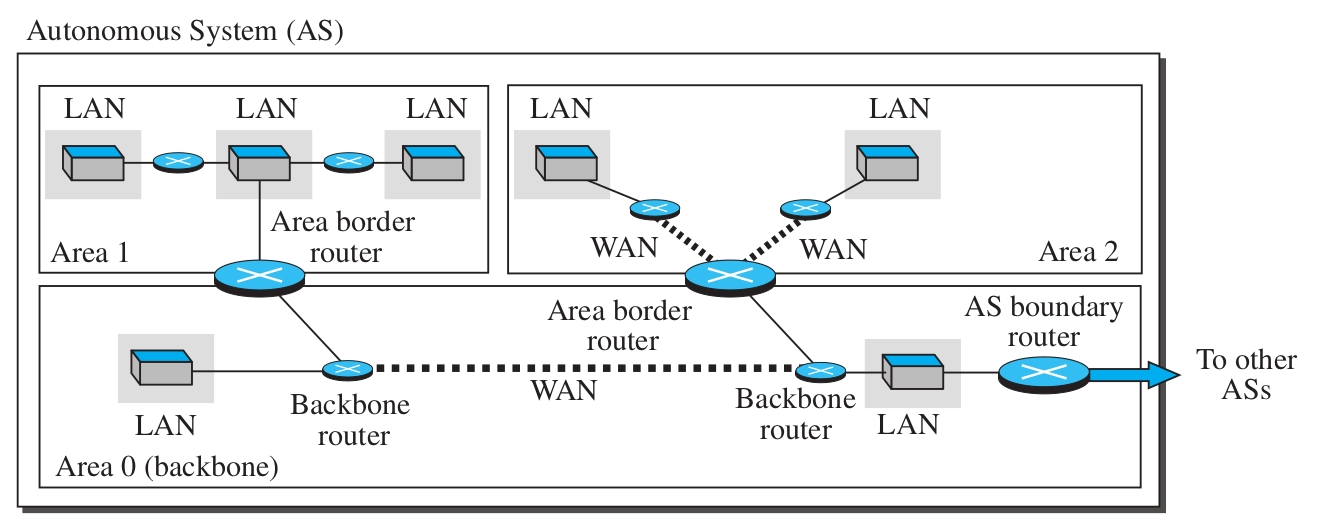
\includegraphics[width=0.9\linewidth]{ospf}
	\caption{Autonomous System Hierarchy}
	\label{net2}
\end{figure}

\section{section1}
\lipsum[2] % Please comment this line and type in the introduction chapter


\subsection{title 2}
\lipsum[3] % Please comment this line and type in the introduction chapter

\noindent The system is described by the equation \ref{sys_eq1} below. Here y is the ordinate and x is the abscissa , m is the slope and c a constant.

\begin{equation} \label{sys_eq1}
y = mx + c
\end{equation}

\noindent Page centered and unnumbered multiple equations. The * symbol supresses equation numbering.
% Page centered and unnumbered equations
\begin{align*}
2x - 5y &=  8 \\ 
3x + 9y &=  -12

\end{align*}

\noindent Side by side figures can be created using this environment. See fig \ref{wave} below.
\begin{figure}[h!]
	\centering
	\begin{subfigure}[b]{0.4\textwidth}
		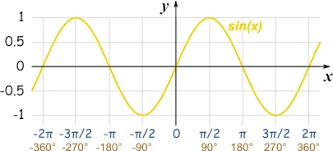
\includegraphics[width=\textwidth]{sinewave}
		\caption{Sine Wave}
		\label{fig:1}
	\end{subfigure}
	\hspace{20mm}
	\begin{subfigure}[b]{0.4\textwidth}
		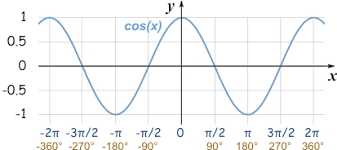
\includegraphics[width=\linewidth]{cosine}
		\caption{Cosine Wave}
		\label{fig:2}
	\end{subfigure}
\caption{The Sine and Cosine waves}
\label{wave}
\end{figure}

	
\begin{table}[h!]
	\centering
	\caption{test table}
	\vspace*{5pt}
	\begin{tabular}{|c|c|c|}
		\hline
		Sl. No & Item 1 & Itm 2 \\ \hline
		1      & 37     & 45    \\ \hline
		2      & 42     & 23    \\ \hline
		3      & 47     & 1     \\ \hline
		4      & 52     & -21   \\ \hline
		5      & 57     & -43   \\ \hline
		6      & 62     & -65   \\ \hline
		7      & 67     & -87   \\ \hline
		8      & 72     & -109  \\ \hline
		9      & 77     & -131  \\ \hline
		10     & 82     & -153  \\ \hline
	\end{tabular}
\end{table}
%%********************Chapter 4**********
\chapter{Result and Discussion}

\lipsum[2] 
%%********************Chapter 5**********
\chapter{Conclusion and Future work}

\lipsum[2] 

%%********************References**********
%%****This template uses IEEE bibliography style
% The bib file references.bib can be found in the folder. Include the references in the bib file in BibTeX format. A quick video to generate the BibTeX file can be found at   % http://bit.ly/bibtex7
%
\bibliography{references}
\newpage

% Please check the Reference config section (in the preamble) of this file if your references are not cited properly.
\end{document}